\begin{comment}
\end{comment}

\chapter{Algorithmes variationnels quantiques}

%-----------------------------------------------------------------------------%

\begin{comment}
\subsection*{Plan}

\begin{enumerate}
    \item Décrire les algorithmes variationels en général (algorithmes hybrides)
    \item Expliquer les objectifs de ces algorithmes
    \item Expliquer les avantages (exemple: algorithmes à court-terme, qubits bruités, NISQ)
    \item Expliquer la chronologie avec les QAOA
    \item Expliquer comment est-ce qu'on peut utiliser ceux-ci comme générateur pour l'algorithme JVV.
    \item Pourquoi est-ce que QAOA est une approche non-locale?
\end{enumerate}
    
\subsection*{Références}

1. Cerezo, M. et al. Variational quantum algorithms. Nat Rev Phys 3, 625–644 (2021).

2. Bharti, K. et al. Noisy intermediate-scale quantum (NISQ) algorithms. Rev. Mod. Phys. 94, 015004 (2022).
\end{comment}

\textcolor{mydarkred}{\textit{Ajouter un dessin.}}

\textcolor{mydarkred}{\textit{Importance des heuristiques quantiques (voir qaoa (2e version) paper)}}

%-----------------------------------------------------------------------------%

\section{Approche adiabatique quantique}
% \section{Algorithme adiabatique quantique}

\begin{comment}
\subsection{Plan}

\begin{enumerate}
    \item QAA est adiabatique alors que QAOA est contre-adiabatique.
\end{enumerate} 
\end{comment}

Le \textit{théorème adiabatique}, introduit par Born et Fock~\cite{bornBeweisAdiabatensatzes1928}, peut être énoncé simplement comme suit:

\begin{subtheorem}{Théorème adiabatique~\cite{bornBeweisAdiabatensatzes1928}}{theoreme-adiabatique}
    Un système physique demeure dans son état propre instantané si une perturbation donnée agit sur lui suffisament lentement et s'il y a un intervalle significatif entre la valeur propre et le reste du spectre de l'Hamiltonien.
\end{subtheorem}

Bien que différentes versions de ce théorème furent rigoureusement formulées~\cite{albashAdiabaticQuantumComputing2018}, une version approximative de celui-ci, proposée par Messiah~\cite{messiahQuantumMechanics1999} et rectifiée par Amin~\cite{aminConsistencyAdiabaticTheorem2009}, est présentée ici dans l'objectif d'élucider les mécanismes du théorème. Un système quantique, décrit par un Hamiltonien dépendant du temps $H(t)$, évolue selon l'équation de Schrödinger

% , en commençant par Kant en 1950~\cite{katoAdiabaticTheoremQuantum1950},

\begin{align*}
   i \hbar \frac{\partial \ket{\psi(t)}}{\partial t} = H(t) \ket{\psi} \,.
\end{align*}

Considérons ici que l'Hamiltonien $H(t)$ peut s'écrire sous la forme $H(t) = \tilde{H}(s)$, où $s=t/T \in [0,1]$ est le temps adimensionnel, de manière à ce que $T$ contrôle le taux de variation dans le temps de $H(t)$. Soit $\ket{\varepsilon_{j} (s)}$ les états propres instantanés de $\tilde{H}(s)$ avec énergie $\varepsilon_{j}$ (potentiellement dégénérée) tel que

\begin{equation}
   \tilde{H}(s) \ket{\varepsilon_{j}(s)} = \varepsilon_{j}(s) \ket{\varepsilon_{j}(s)} \,,
\end{equation}

où $\varepsilon_{j}(s) < \varepsilon_{j+1}(s) \ \forall j,s$ et $j \in \set{ 0, 1, 2, \dots }$. L'approximation adiabatique indique qu'un état initial préparé dans un des états propres instantanés $\ket{\varepsilon_{j}(0)}$ demeure dans le même état propre instantané $\ket{\varepsilon_{j}(t)}$ à une phase globale près si $\varepsilon_{i}(s) - \varepsilon_{j}(s) \neq  0$ et

\begin{equation}
    T \gg \max_{s \in [0,1]} \frac{\lvert \braket{ \varepsilon_{i}(s) | \partial_{s} \tilde{H}(s) | \varepsilon_{j}(s) } \rvert }{\lvert \varepsilon_{i}(s) - \varepsilon_{j}(s) \rvert^{2} } \ \forall j \neq i \,.
\end{equation}

\textcolor{mydarkred}{\textit{Rajouter une intuition et un lien avec le théorème.}}

L'approximation adiabatique est souvent utilisée à partir de l'état fondamental $\ket{\varepsilon_{0}(t)}$, menant à la définition du gap spectral entre l'état fondamental et le premier état excité du système $\Delta(s) = \varepsilon_{1}(s) - \varepsilon_{0}(s)$. Généralement, le maximum de $\braket{ \varepsilon_{i}(s) | \partial_{s} \tilde{H}(s) | \varepsilon_{j}(s)}$ est de l'ordre d'une valeur propre typique de $\tilde{H}$ et petit. Le minimum du carré de l'inverse du gap spectral $\Delta$ constitue alors un critère pratique pour quantifier le temps nécessaire à l'évolution adiabatique. \textcolor{mydarkred}{\textit{Reformuler et faire attention aux symboles.}}

L'algorithme adiabatique quantique, introduit par Farhi~\cite{farhiQuantumComputationAdiabatic2000}, emploie un ordinateur quantique physique pour la résolution de problèmes d'optimisation combinatoire en se basant sur le théorème adiabatique quantique. Pour ce faire, le système physique est initialement préparé dans l'état fondamental d'un Hamiltonien de forçage $H_{D}$ facile à construire et dont l'état fondamental est simple à trouver. La solution du problème, encodée dans l'état fondamental de l'Hamiltonien de problème $H_{P}$, est alors obtenue en transitionnant de l'Hamiltonien $H_{D}$ à l'Hamiltonien $H_{P}$ par une évolution adiabatique. Plus précisément, l'Hamiltonien du système s'écrit comme


\begin{equation}
    \tilde{H}(s) = \left(1-s\right) H_{D} + s H_{P} \,.
\end{equation}

Ainsi, en assumant que le gap spectral entre l'état fondamental et l'état excité est non-nul, la solution du problème est toujours obtenue si l'évolution est suffisamment lente tel que guarantit par le théorème adiabatique quantique.

\textcolor{mydarkred}{\textit{Mais est-ce que le gap en non-nul en général?}}

\textcolor{mydarkred}{\textit{Tradeoff entre temps et success probability.}}

Cet algorithme partage plusieurs similitudes avec l'algorithme quantique d'optimisation approximative qui seront explorées dans les prochaines sections. \textcolor{mydarkred}{\textit{...}}

\textcolor{mydarkred}{\textit{Parler du recuit quantique?}}

\textcolor{mydarkred}{\textit{Ajouter un dessin.}}


%-----------------------------------------------------------------------------%

\section{Algorithme quantique d'optimisation approximative}

\begin{comment}
\subsection*{Plan}
    
\begin{enumerate}
    \item Expliquer l'histoire et le lien avec le recuit quantique
\end{enumerate}

\subsection*{Références}

1. Farhi, E., Goldstone, J. and Gutmann, S. A Quantum Approximate Optimization Algorithm. Preprint at https://doi.org/10.48550/arXiv.1411.4028 (2014).

2. Kadowaki, T. and Nishimori, H. Quantum annealing in the transverse Ising model. Phys. Rev. E 58, 5355–5363 (1998).

3. Finnila, A. B., Gomez, M. A., Sebenik, C., Stenson, C. and Doll, J. D. Quantum annealing: A new method for minimizing multidimensional functions. Chemical Physics Letters 219, 343–348 (1994).

4. Farhi, E. et al. A Quantum Adiabatic Evolution Algorithm Applied to Random Instances of an NP-Complete Problem. Science 292, 472–475 (2001).

5. Farhi, E., Goldstone, J., Gutmann, S. and Sipser, M. Quantum Computation by Adiabatic Evolution. Preprint at https://doi.org/10.48550/arXiv.quant-ph/0001106 (2000).

6. Parler la adiabatic quantum computation https://arxiv.org/abs/1611.04471
\end{comment}

Bien que le calcul adiabatique quantique soit utilisé pour résoudre les problèmes d'optimisation combinatoire (\textcolor{mydarkred}{\textit{Source?}}), le temps nécessaire pour une évolution adiabatique constitue un facteur limitant pour de nombreux problèmes. L'\textit{algorithme quantique d'optimisation approximative} (QAOA)~\cite{farhiQuantumApproximateOptimization2014} propose ainsi une alternative, un raccourci à l'adiabacité: la contre-diabacité.

%-----------------------------------------------------------------------------

\subsection{Description de l'algorithme}
\label{subsec:description-algorithme}

\begin{comment}
subsection*{Plan}
    
\begin{enumerate}
    \item Décrire le \textit{Quantum Approximate Optimization Algorithm}
    \item QAOA sees the whole graph?
    \item avantage vs les algorithmes classiques?
\end{enumerate}

\subsection*{Références}

1. Farhi, E., Goldstone, J. and Gutmann, S. A Quantum Approximate Optimization Algorithm. Preprint at https://doi.org/10.48550/arXiv.1411.4028 (2014).
\end{comment}

L'algorithme quantique d'optimisation approximative, étant une idée prometteuse pour les applications des ordinateurs quantiques, a mené à une quantité incroyable de travaux dans les précédentes années. Ainsi, pour simplifier la compréhension de ce concept, l'algorithme original, dû à Farhi~\cite{farhiQuantumApproximateOptimization2014}, est d'abord présenté.

QAOA repose sur deux différents Hamiltoniens: l'Hamiltonien de problème $H_{P}$ et l'Hamiltonien de forçage $H_{D}$. \textcolor{mydarkred}{\textit{Drive, mixer, problem, phase?}} L'Hamiltonien de problème est formulé de façon à encoder la solution, potentiellement dégénérée, du problème d'optimisation combinatoire dans son état fondamental. L'Hamiltonien de forçage, quant à lui, est donné par

\begin{equation}
    \label{eq:x-drive}
    H_{D} = \sum_{i=1}^{n} X_{i} \,,
\end{equation}

où $X_{i}$ est l'opérateur de Pauli $X$ appliqué sur le qubit $i$ d'un système à $n$ qubits. L'Hamiltonien de forçage est construit de manière à induire de l'interférence et ainsi permettre l'exploration de l'espace d'Hilbert. 

Par définition, l'Hamiltonien $H_{p}$ est diagonal dans la base computationnelle, alors que l'Hamiltonien $H_{D}$ comprend des termes hors-diagonaux. Deux opérations unitaires paramétrées sont définies à partir des Hamiltoniens $H_{P}$ et $H_{D}$: l'opérateur de problème $U_{P}(\gamma) = e^{-i \gamma H_{P}}$ ainsi que l'opérateur de forçage $U_{D}(\beta) = e^{-i \beta H_{D}}$. L'opérateur $U_{P}$ représente une rotation de phase, paramétrisée par $\gamma$, des états de la base computationnelle dépendamment de leur énergie donné par $H_{P}$. L'opérateur $U_{D}$, paramétrisé par $\beta$, superpose différents états de la base computationnel ayant précédamment acquéri différents facteurs de phase, menant ainsi à de l'interférence.

En tant que VQA, QAOA est un algorithme hybride composé d'un circuit quantique paramétré et d'un optimiseur classique. Le circuit quantique est d'abord préparé dans un état propre de l'Hamiltonien de forçage. Pour l'Hamiltonien~\ref{eq:x-drive}, un exemple d'état initial possible serait $\ket{\psi_{0}} = \ket{+}^{\otimes n}$. Le produit des opérateurs $U_{D}U_{P}$ est alors appliqué $p$ fois sur l'état initial $\ket{\psi_{0}}$. L'état obtenu est

\begin{equation}
    \label{eq:final-state}
    \ket{\psi(\vec{\gamma}, \vec{\beta})} = U_D(\beta_p) U_P(\gamma_p) \cdots U_D(\beta_1) U_P(\gamma_1) \ket{\psi_{0}} \,.
\end{equation}

où $\vec{\gamma} = (\gamma_{1}, \dots, \gamma_{p})$ et $\vec{\beta} = (\beta_{1}, \dots, \beta_{p})$. Une fois l'état $\ket{\psi(\vec{\gamma}, \vec{\beta}})$ préparé, la valeur moyenne de l'énergie, donnée par

\begin{equation}
    E_{P} (\vec{\gamma}, \vec{\beta}) = \braket{ \psi(\vec{\gamma}, \vec{\beta}) | H_{P} | \psi(\vec{\gamma}, \vec{\beta}) } \,,
\end{equation}

est mesurée. 

\textcolor{mydarkred}{\textit{Ajouter une figure.}}

\textcolor{mydarkred}{\textit{Level crossings?}}

\textcolor{mydarkred}{\textit{Écrire un algorithme?}}

%-----------------------------------------------------------------------------%

\subsubsection{Préparation de l'état initial}
\label{subsec:encodage-probleme}

\textcolor{mydarkred}{\textit{Est-ce que l'état initial doit être dans un état propre de l'Hamiltonien de forçage?}}

%-----------------------------------------------------------------------------%

\subsubsection{Encodage du problème}
\label{subsec:encodage-probleme}

\begin{comment}
\subsection*{Plan}

\begin{enumerate}
    \item Introduire la fonction de coût
    \item Introduire le modèle d'Ising et le modèle QUBO
    \item Décrire la transformation d'Ising pour NAE3SAT et 1in3SAT
    \item Prouver la transformation d'Ising pour NAE3SAT et 1in3SAT
\end{enumerate}

\subsection*{Références}

1. Lucas, A. Ising formulations of many NP problems. Frontiers in Physics 2, (2014).
2. MAPPING NP-HARD AND NP-COMPLETE OPTIMISATION PROBLEMS
TO QUADRATIC UNCONSTRAINED BINARY OPTIMISATION PROBLEMS. (CORRECTION DE 1)

\end{comment}

Comment est-ce qu'un problème d'optimisation combinatoire $\varphi(x):\set{ 0, 1 }^{\otimes n} \to \set{ 0, 1 }$ peut être encodé par un Hamiltonien $H_{P}$? D'abord, les entrées $x = x_{1} \dots x_{n}$ du problème sont caractérisées par une fonction de coût $C(x):\set{ +1, -1 }^{\otimes n} \to \mathbb{R}_{\geq 0}$. Une entrée optimale est associée à un coût nul, alors qu'une entrée non-optimale est associée à un coût positif, en fonction de son optimalité. Résoudre le problème correspond alors à trouver l'entrée optimale, c'est-à-dire l'entrée $x^{*}$ minimisant la fonction de coût. L'Hamiltonien de problème se définit alors par

\begin{equation}
    H_{P} \ket{x} = C(x) \ket{x}
\end{equation}

Cette équation implique que l'état fondamental de l'Hamiltonien $H_{P}$ encode les solutions au problème donné. 

\textcolor{mydarkred}{\textit{Parler de QUBO.}}

\textcolor{mydarkred}{\textit{Il s'agit donc de terms de pénalités.}}


Comme trouver l'état fondamental d'un modèle d'Ising constitue un problème NP, il existe alors nécessairement une réduction entre ce problème et les différents problèmes NP. Bien que ces réductions ne sont pas nécessairement évidentes, plusieurs de celles-ci ont été formulées pour le recuit quantique~\cite{lucasIsingFormulationsMany2014,lodewijksMappingNPhardNPcomplete2020} \textcolor{mydarkred}{\textit{recuit ou AQO?}}. Un réduction intéressante relie le problème positif NAE3SAT au modèle d'Ising antiferromagnétique. Soit la formule propositionelle $f(x_{1}, x_{2}, x_{3}) = (x_{1} \lor x_{2} \lor x_{3})$. En associant chaque variable $x_{i}$ à un spin $\sigma_{i}$, cette formule se réduit à un modèle d'Ising en considérant un réseau triangulaire composé des spins $\sigma_{i}$, où chacun de ceux-ci sont reliés aux deux autres spins. L'Hamiltonien d'un tel modèle est donné par

\begin{equation}
    H_{P} = \sigma_{1}\sigma_{2} + \sigma_{2}\sigma_{3} + \sigma_{3}\sigma_{1}
\end{equation}

Les énergies associées à chaque combinaison possible des spins sont présentés dans le tableau~\ref{tab:energie-nae3sat}, où les spins vers le haut sont représentés par 0 et les spins vers le bas sont représentés par 1. La frustration des spins sur le réseau implique que les seuls états qui ne sont pas dans l'état fondamental sont les états $000$ et $111$. Hors, il s'agit des deux combinaisons ne faisant pas partie de l'ensemble des solutions du problème positif NAE3SAT.


\begin{table*}[h]
    \centering
    \begin{subtable}{0.4\textwidth}
        \centering
        \begin{tabular}{c c}
            \hline
            Entrée & Énergie \\
            \hline
            000 & 3 \\
            001 & -1 \\
            010 & -1 \\
            100 & -1 \\
            011 & -1 \\
            110 & -1 \\
            101 & -1 \\
            111 & 3 \\
            \hline
        \end{tabular}
        \caption{}
        \label{tab:energie-nae3sat}
    \end{subtable}
    % \hspace*{4em}
    \begin{subtable}{0.4\textwidth}
        \centering
        \begin{tabular}{c c}
            \hline
            Entrée & Énergie \\
            \hline
            000 & 0 \\
            001 & -2 \\
            010 & -2 \\
            100 & -2 \\
            011 & 0 \\
            110 & 0 \\
            101 & 0 \\
            111 & 6 \\
            \hline
        \end{tabular}
        \caption{}
        \label{tab:energie-1in3sat}
    \end{subtable}
    \caption{Énergie de chaque entrée dans le modèle d'Ising pour le problème NAE3SAT (a) et 1-in-3SAT (b).}
\end{table*}

Plus généralement, tous les problèmes positif NAE3SAT sont représentables par un modèle d'Ising en appliquant la transformation précédente sur chacune des clauses de la formule, tel qu'illustré à la figure~\ref{fig:transformation-ising}, donnant ainsi l'Hamiltonien 

\begin{equation}
    H_P = - \sum_{(i,j) \in E} J_{ij} \sigma_i \sigma_j - \sum_{i \in V} h_i \sigma_i \,.
\end{equation}

où $E$ est l'ensemble d'arrêtes et $V$ est l'ensemble de sommets.

\begin{figure}[h]
    \centering
    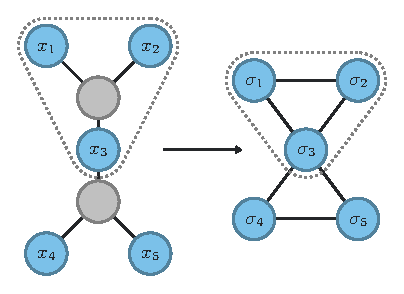
\includegraphics[width=0.55\textwidth]{figures/ising-mapping}
    \caption{}
    \label{fig:transformation-ising}
\end{figure}


%-----------------------------------------------------------------------------%

\subsubsection{Choix du forçage}

\begin{comment}
\subsection*{Plan}

\begin{enumerate}
    \item Expliquer le but du forçage
    \item Expliquer forçage en X
    \item Expliquer le forçage de Grover
    \item Énumérer les forçages populaires
    \item Est-ce que le mixer doit être un vecteur propre de l'état initial?
\end{enumerate}

\subsection*{Références}
\end{comment}

\textcolor{mydarkred}{\textit{Les mixers peuvent être utilisés pour restreindre l'espace.}}


\textcolor{mydarkred}{\textit{Toute la dépendance au problème doit être encodée dans $H_P$ pour le QA, alors que pas nécessairement ici.}}

%-----------------------------------------------------------------------------%

\subsection{Contre-diabacité}

\begin{comment}
    \begin{itemize}
        \item Contre-diabacité
        \item Trottérisation
    \end{itemize}
\end{comment}


\textcolor{mydarkred}{\textit{Expliquer la contre-diabacité.}}

\textcolor{mydarkred}{\textit{Expliquer la trotterisation (voir citation dans notre papier).}}

\textcolor{mydarkred}{\textit{Parler de QAOA lorsque $p \to \infty$}}


%-----------------------------------------------------------------------------%

\section{Approche quantique des opérateurs alternants}

\begin{comment}
\subsection*{Plan}

\begin{enumerate}
    \item Décrire le \textit{Quantum Alternating Operator Ansatz}
    \item Décrire \textit{Grover-Mixer Quantum Alternating Operator Ansatz}
\end{enumerate}

\subsection*{Références}

1. Hadfield, S. et al. From the Quantum Approximate Optimization Algorithm to a Quantum Alternating Operator Ansatz. Algorithms 12, 34 (2019).

2. Bärtschi, A. and Eidenbenz, S. Grover Mixers for QAOA: Shifting Complexity from Mixer Design to State Preparation. in 2020 IEEE International Conference on Quantum Computing and Engineering (QCE) 72–82 (2020). doi:10.1109/QCE49297.2020.00020.
\end{comment}

L'algorithme quantique d'optimisation approximative applique en alternance un Hamiltonien de problème et un Hamiltonien de forçage, guidé par l'approche quantique adiabatique. Cet algorithme comporte une limitation importante: les opérateurs appliqués doivent être sous la forme d'une évolution temporelle d'un Hamiltonien local fixe. Cette restriction entrave la construction d'opérateurs unitaires potentiellement plus efficaces.

L'\textit{approche quantique des opérateurs alternants} (QAOA), introduit par Hadfield et al.~\cite{hadfieldQuantumApproximateOptimization2019}, généralise l'algorithme quantique d'optimisation approximative en permettant l'alternance de familles générales d'opérateurs unitaires paramétrisés plutôt qu'uniquement des opérateurs basés sur un Hamiltonien. Cet ansatz supporte ainsi la représentation d'une plus grand nombre d'états, pouvant possiblement être construit de manière plus efficace.

L'algorithme quantique d'approximation quantique et l'approche quantique des opérateurs alternants possèdent le même acronyme. Comme cette dernière étend le premier, l'acronyme QAOA fera référence à l'approche quantique des opérateurs alternant pour le reste de la présente section.

Cette extension trouve son utilité principalement dans la création d'opérateurs de forçage. Restreindre l'espace des configurations d'un problème selon les contraintes de celui-ci permet d'éviter .


%-----------------------------------------------------------------------------%

\subsection{Description de l'approche}

%-----------------------------------------------------------------------------%




\subsection{Forçage de Grover}

\begin{equation}
    U_D^{\mathrm{Grover}} = U_{S}\left[ \mathds{1} -\left(1-e^{-i \beta}\right) (\ket{0}\!\bra{0})^{\otimes n} \right] U_{S}^{\dagger} \,,
\end{equation}



%-----------------------------------------------------------------------------%

\section{Configuration des paramètres}
\label{subsec:initialisation-parametres}

\begin{comment}
\subsection*{Plan}

\begin{enumerate}
    \item Décrire l'importance d'une bonne initialisation des paramètres (\textit{barren plateau}, non-convexité des paramètres)
    \item Énumérer les principales méthodes
    \item Expliquer l'initialisation aléatoire par grille
    \item Expliquer \textit{TQA}
\end{enumerate}

\subsection*{Références}

1. Bittel, L. and Kliesch, M. Training Variational Quantum Algorithms Is NP-Hard. Phys. Rev. Lett. 127, 120502 (2021).

2. Anschuetz, E. R. and Kiani, B. T. Beyond Barren Plateaus: Quantum Variational Algorithms Are Swamped With Traps. Nat Commun 13, 7760 (2022).

3. Akshay, V., Philathong, H., Morales, M. E. S. and Biamonte, J. D. Reachability Deficits in Quantum Approximate Optimization. Phys. Rev. Lett. 124, 090504 (2020).
    
4. Cain, M., Farhi, E., Gutmann, S., Ranard, D. and Tang, E. The QAOA gets stuck starting from a good classical string. Preprint at https://doi.org/10.48550/arXiv.2207.05089 (2022).

Peut-être une référence de plus qui traite directement des barrens plateau?
\end{comment}

L'optimisation classique des paramètres de QAOA 


%-----------------------------------------------------------------------------%

\section{Échantillonage et biais}

\subsection*{Plan}

\begin{enumerate}
    \item Expliquer l'importance de l'échantillonnage non-biaisé
    \item Expliquer le problème d'échantillonage associé au recuit quantique
    \item Expliquer le problème d'échantillonage associé à QAOA
    \item Expliquer pourquoi GM-QAOA résout ce problème (ne pas oublier d'expliquer les inconvénients de cette méthode)
\end{enumerate}

\subsection*{Références}

1. Zhang, Z. et al. Grover-QAOA for 3-SAT: Quadratic Speedup, Fair-Sampling, and Parameter Clustering. Preprint at https://doi.org/10.48550/arXiv.2402.02585 (2024).

2. Mandrà, S., Zhu, Z. and Katzgraber, H. G. Exponentially Biased Ground-State Sampling of Quantum Annealing Machines with Transverse-Field Driving Hamiltonians. Phys. Rev. Lett. 118, 070502 (2017).

3. Matsuda, Y., Nishimori, H. and Katzgraber, H. G. Ground-state statistics from annealing algorithms: quantum versus classical approaches. New J. Phys. 11, 073021 (2009).

Plus de sources sur le fair sampling pour QAOA?
